%-----------------------------------------------%
% Início do plano de aula
%-----------------------------------------------%
\thispagestyle{empty}
\begin{center}
	\begin{minipage}[!]{\linewidth}
        \begin{minipage}[!]{.19\linewidth}
            
\includegraphics[width=\linewidth]{img/logo.png}           
        \end{minipage}
        \begin{minipage}[!]{.8\linewidth}
            \center
            \ABNTEXchapterfont\normalsize\MakeUppercase{\imprimirinstituicao}
            \par
            \vspace*{10pt}                     
            \ABNTEXchapterfont\normalsize\MakeUppercase{\centro}
            \par
            \vspace*{10pt}           
            \ABNTEXchapterfont\normalsize\MakeUppercase{\disciplina}
        \end{minipage}        
    \end{minipage}
    \\ \vspace{0.5cm}
    \rule{\textwidth}{.5pt}   
\end{center}
    \textual
    \begin{center}
      \section{Teoria Corpuscular da Luz}
      \par
    \end{center}
    
    \noindent \textbf{Estagiário(a): }\imprimirautor 
    
    \noindent \textbf{U.E.:} EEB Giovani Pasqualini Faraco
    
    \noindent \textbf{Série:} 2º Ano\hfill{}\textbf{Turma: }2º--5
    
    \noindent \textbf{Aula:} 003\hfill{}\textbf{Data:} 21/10/2022\hfill{}\textbf{Duração:} $45\min$
    \rule{\textwidth}{.5pt}
    \bigskip{}  
    

    \noindent
    \begin{center}
      \textbf{O Modelo Corpuscular Newtonianao para a Luz}
    \par\end{center}

    \noindent \textbf{Resumo da aula:} Nesta aula será apresentado o modelo corpuscular da luz na concepção newtoniana. Os fenômenos de reflexão e refração da luz serão deduzidos bem como seus pressupostos.

    \par\noindent \textbf{Habilidades BNCC:} EM13CNT201.
    
    \vspace*{30pt}
    \subsection*{Objetivo de Aprendizagem}
    \begin{itemize}
        \item Compreender os fundamentos do modelo corpuscular da luz e suas principais proposições;
    \end{itemize}
    \medskip{}
    \vspace*{50pt}
    
    \noindent \textbf{Núcleo Conceitual:} \emph{Teoria corpuscular da luz; reflexão e refração.}

    \newpage

    \section*{Procedimento Didático} 
    \noindent \emph{1º Momento:} O mecanicismo newtoninano. 
	\par\noindent\rule{.3\textwidth}{.5pt}  
    \par\noindent \textbf{Tempo previsto:} 10 minutos  

    \noindent \textbf{Dinâmica:} Abrir um diálogo com a turma a repeito do modelo mecanicista. Elucidar que já tiveram bastante contato com este modelo no primeiro ano do ensino médio, na ocasião da cinemática e dinâmica. Deixar claro que este modelo é bastante utilizado nas ciências, nele os fenômenos físicos são explicados por leis do movimentos. Tendo como seus principais defensores, Galileu, Descartes e Newton.

    Newton desenvolveu uma teoria para a luz, baseada na hipótese corpuscular mecanicista, em que a luz é modelada como um feixe de partículas minúsculas sujeitas as leis de movimento que ele mesmo derivou. No entanto, Newton não tinha exata certeza da natureza da luz como destaca o próprio autor
    
    \begin{citacao}
        ``E verdade que, em minha teoria, defendo a corporeidade da luz; mas eu o faço sem uma certeza absoluta, como a palavra talvez dá a entender; e o faço como não mais que uma consequência muito plausível da teoria, não como uma suposição fundamental''\dots \cite{FABIO:2009}
    \end{citacao}

    \vspace{50pt}
    \noindent \emph{2º Momento:} Reflexão corpuscular
	\par\noindent\rule{.3\textwidth}{.5pt}    
    \par\noindent \textbf{Tempo previsto: }15 minutos

    \noindent \textbf{Dinâmica:} Vamos agora ver como Newton explica os fenômenos de reflexão e refração da luz.

    Nesta parte o professor deve fazer sua exposição utilizando o quadro, sempre argumentando e conduzindo os argumentos sem fazer qualquer crítica ao modelo, a ideia é fornecer as bases do pensamento newtoniano para os fenômenos da reflexão e refração na versão corpuscular.

    Iniciar esta exposição, recordando o que foi visto na simulação da aula passada, na reflexão por exemplo, os alunos virão que o ângulo de incidência da luz é sempre igual ao ângulo de reflexão. Será que a teoria corpuscular newtoniana concorda com isso?

    \begin{proof}
        Pra iniciar a demostração ir desenhando no quadro e expondo as ideias a medida que as relações vão aparecendo.
        
        Uma partícula de luz viaja em um meio translúcido com velocidade inicial $\vec{v_0}$ a \autoref{fig:reflexao-newton} a seguir, ilustra a situação antes e depois da partícula colidir com uma interface de separação entre o meio proveniente e um outro meio translúcido qualquer, onde por suposição, não fizemos qualquer restrição aos ângulos de incidência $\theta_i$ e reflexão $\theta_r$
        
        \vspace*{20pt}
        \begin{figure}[!ht]
            \centering
            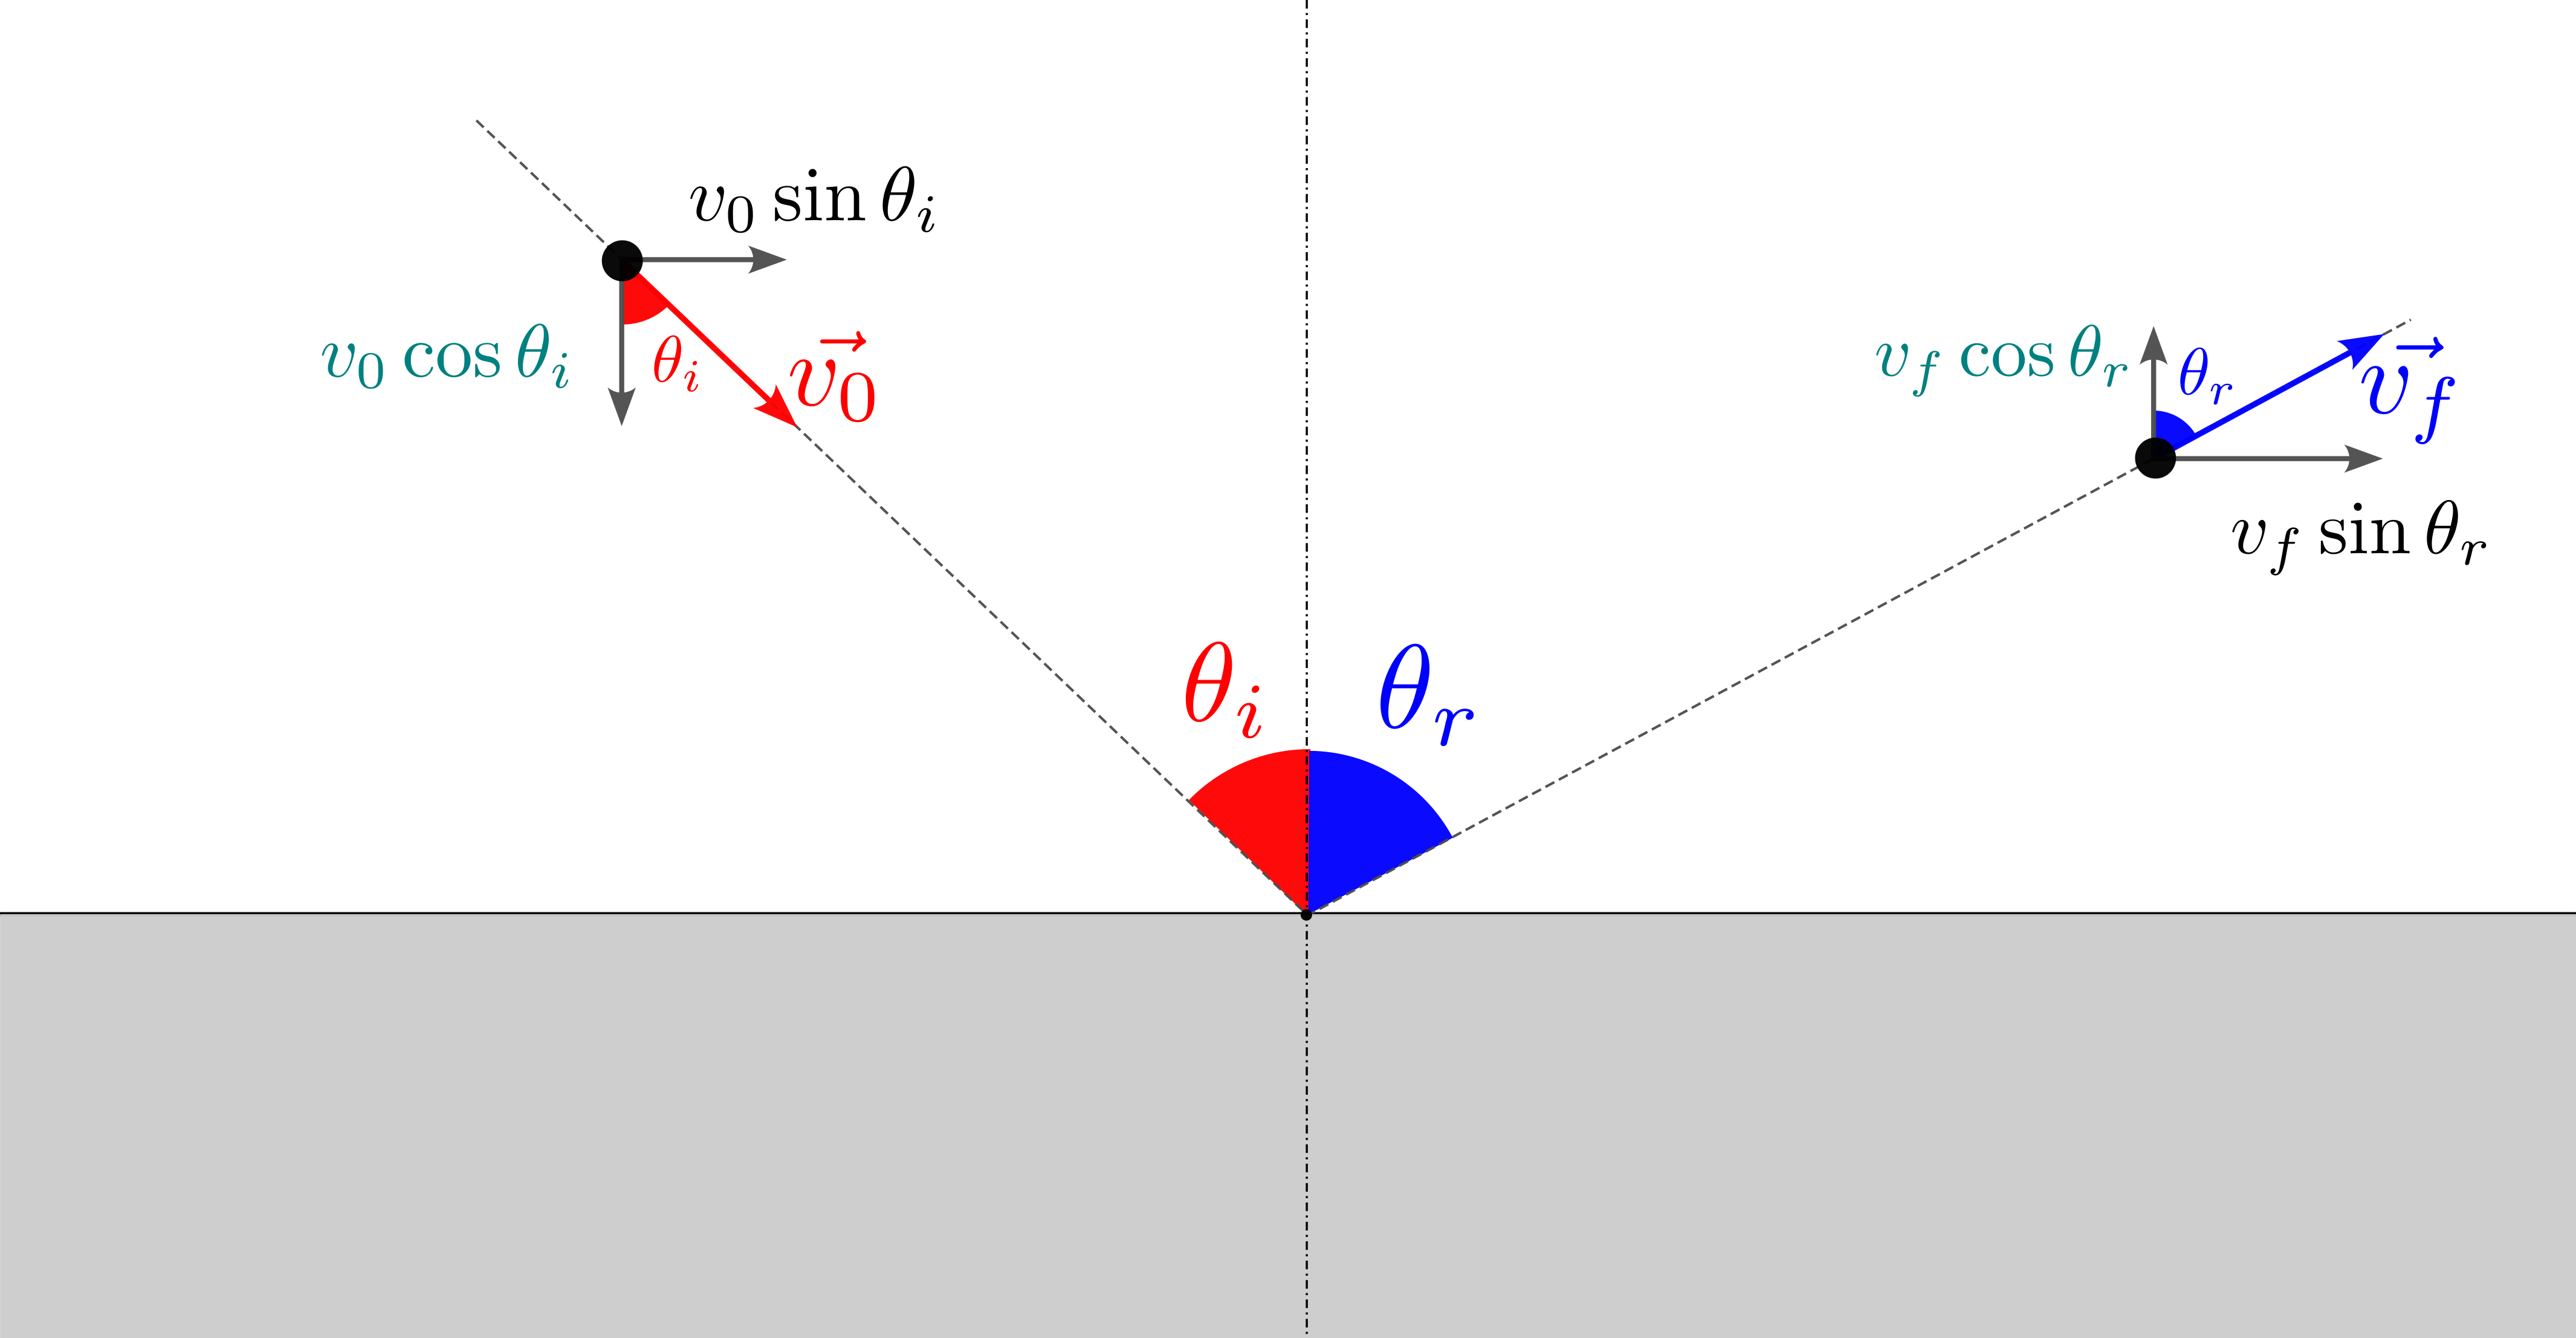
\includegraphics[width=.8\textwidth]{img/reflexao-newton.png}
            \caption{Reflexão corpuscular da luz.}
            \label{fig:reflexao-newton}
        \end{figure}
        \vspace*{20pt}
        
        Supondo que a colisão entre a partícula de luz e a interface seja puramente inelástica, a força resultante que a partícula faz sobre a superfície é normal $\vec{F}_{p,s}$, e pela terceira Lei de Newton a força que a superfície faz sobre a partícula é $-\vec{F}_{s,p}$. Em virtude disto, esta força é responsável por alterar somente a componente vertical da velocidade, mantendo a componente horizontal intacta. O momento linear e a energia são conservados, de maneira que podemos escrever as relações

        \begin{subequations}
            \begin{align}
                \vec{p}_0&=\vec{p}_f\\
                E_0&=E_f
            \end{align}
        \end{subequations}

        \begin{subequations}
            \begin{align}
                mv_0\sin\theta_i&=mv_f\sin\theta_r\label{eq:cons-momento-pla3}\\
                \frac{1}{2}mv_0^2&=\frac{1}{2}mv_f^2\label{eq:cons-energia-pla3}
            \end{align}
        \end{subequations}

        Não havendo dissipação da energia (colisão inelástica) a velocidade final da partícula de luz deve ser igual, em módulo, a velocidade inicial de modo que
        \begin{align}
            \begin{split}
                \sin\theta_i&=\sin\theta_r\\
                \theta_i&=\theta_r
            \end{split}
        \end{align}
    \end{proof}
    Fica assim demostrada a reflexão da luz na teoria corpuscular de Newton

    \vspace{50pt}
    \noindent \emph{3º Momento:} Refração corpuscular
	\par\noindent\rule{.3\textwidth}{.5pt}    
    \par\noindent \textbf{Tempo previsto: }15 minutos

    \noindent \textbf{Dinâmica:} Relembrar o fenômeno da refração observado na simulação, e pegar como exemplo a luz vindo do ar para a água. Os alunos devem lembrar que neste caso, a luz refratada sofre um desvio se aproximando-se da normal à superfície no ponto de contato.

    Vamos agora analisar este fenômeno dentro do ponto de vista da teoria corpuscular newtoniana.

    A exposição feita nesta parte deve seguir de forma semelhar a anterior, fazendo-se sempre argumentações e conduções sem exibir críticas ao modelo.

    \begin{proof}
        Seja uma partícula de luz viajando no ar com velocidade inicial $\vec{v}_0$. Se ao passar de um meio menos denso (ar) para um meio mais denso (água), observa-se uma mudança na trajetória da partícula, de modo tal que sua trajetória no meio mais denso encontra-se mais próximo à normal. Deve atuar, no instante entre a passagem entre os meios, uma força $\vec{F}$ responsável por alterar a componente vertical da partícula nesta direção, a \autoref{fig:refracao-newton} sintetiza a situação antes e depois da partícula de luz entrar na água
        
    \vspace*{20pt}
    \begin{figure}[!ht]
        \centering
        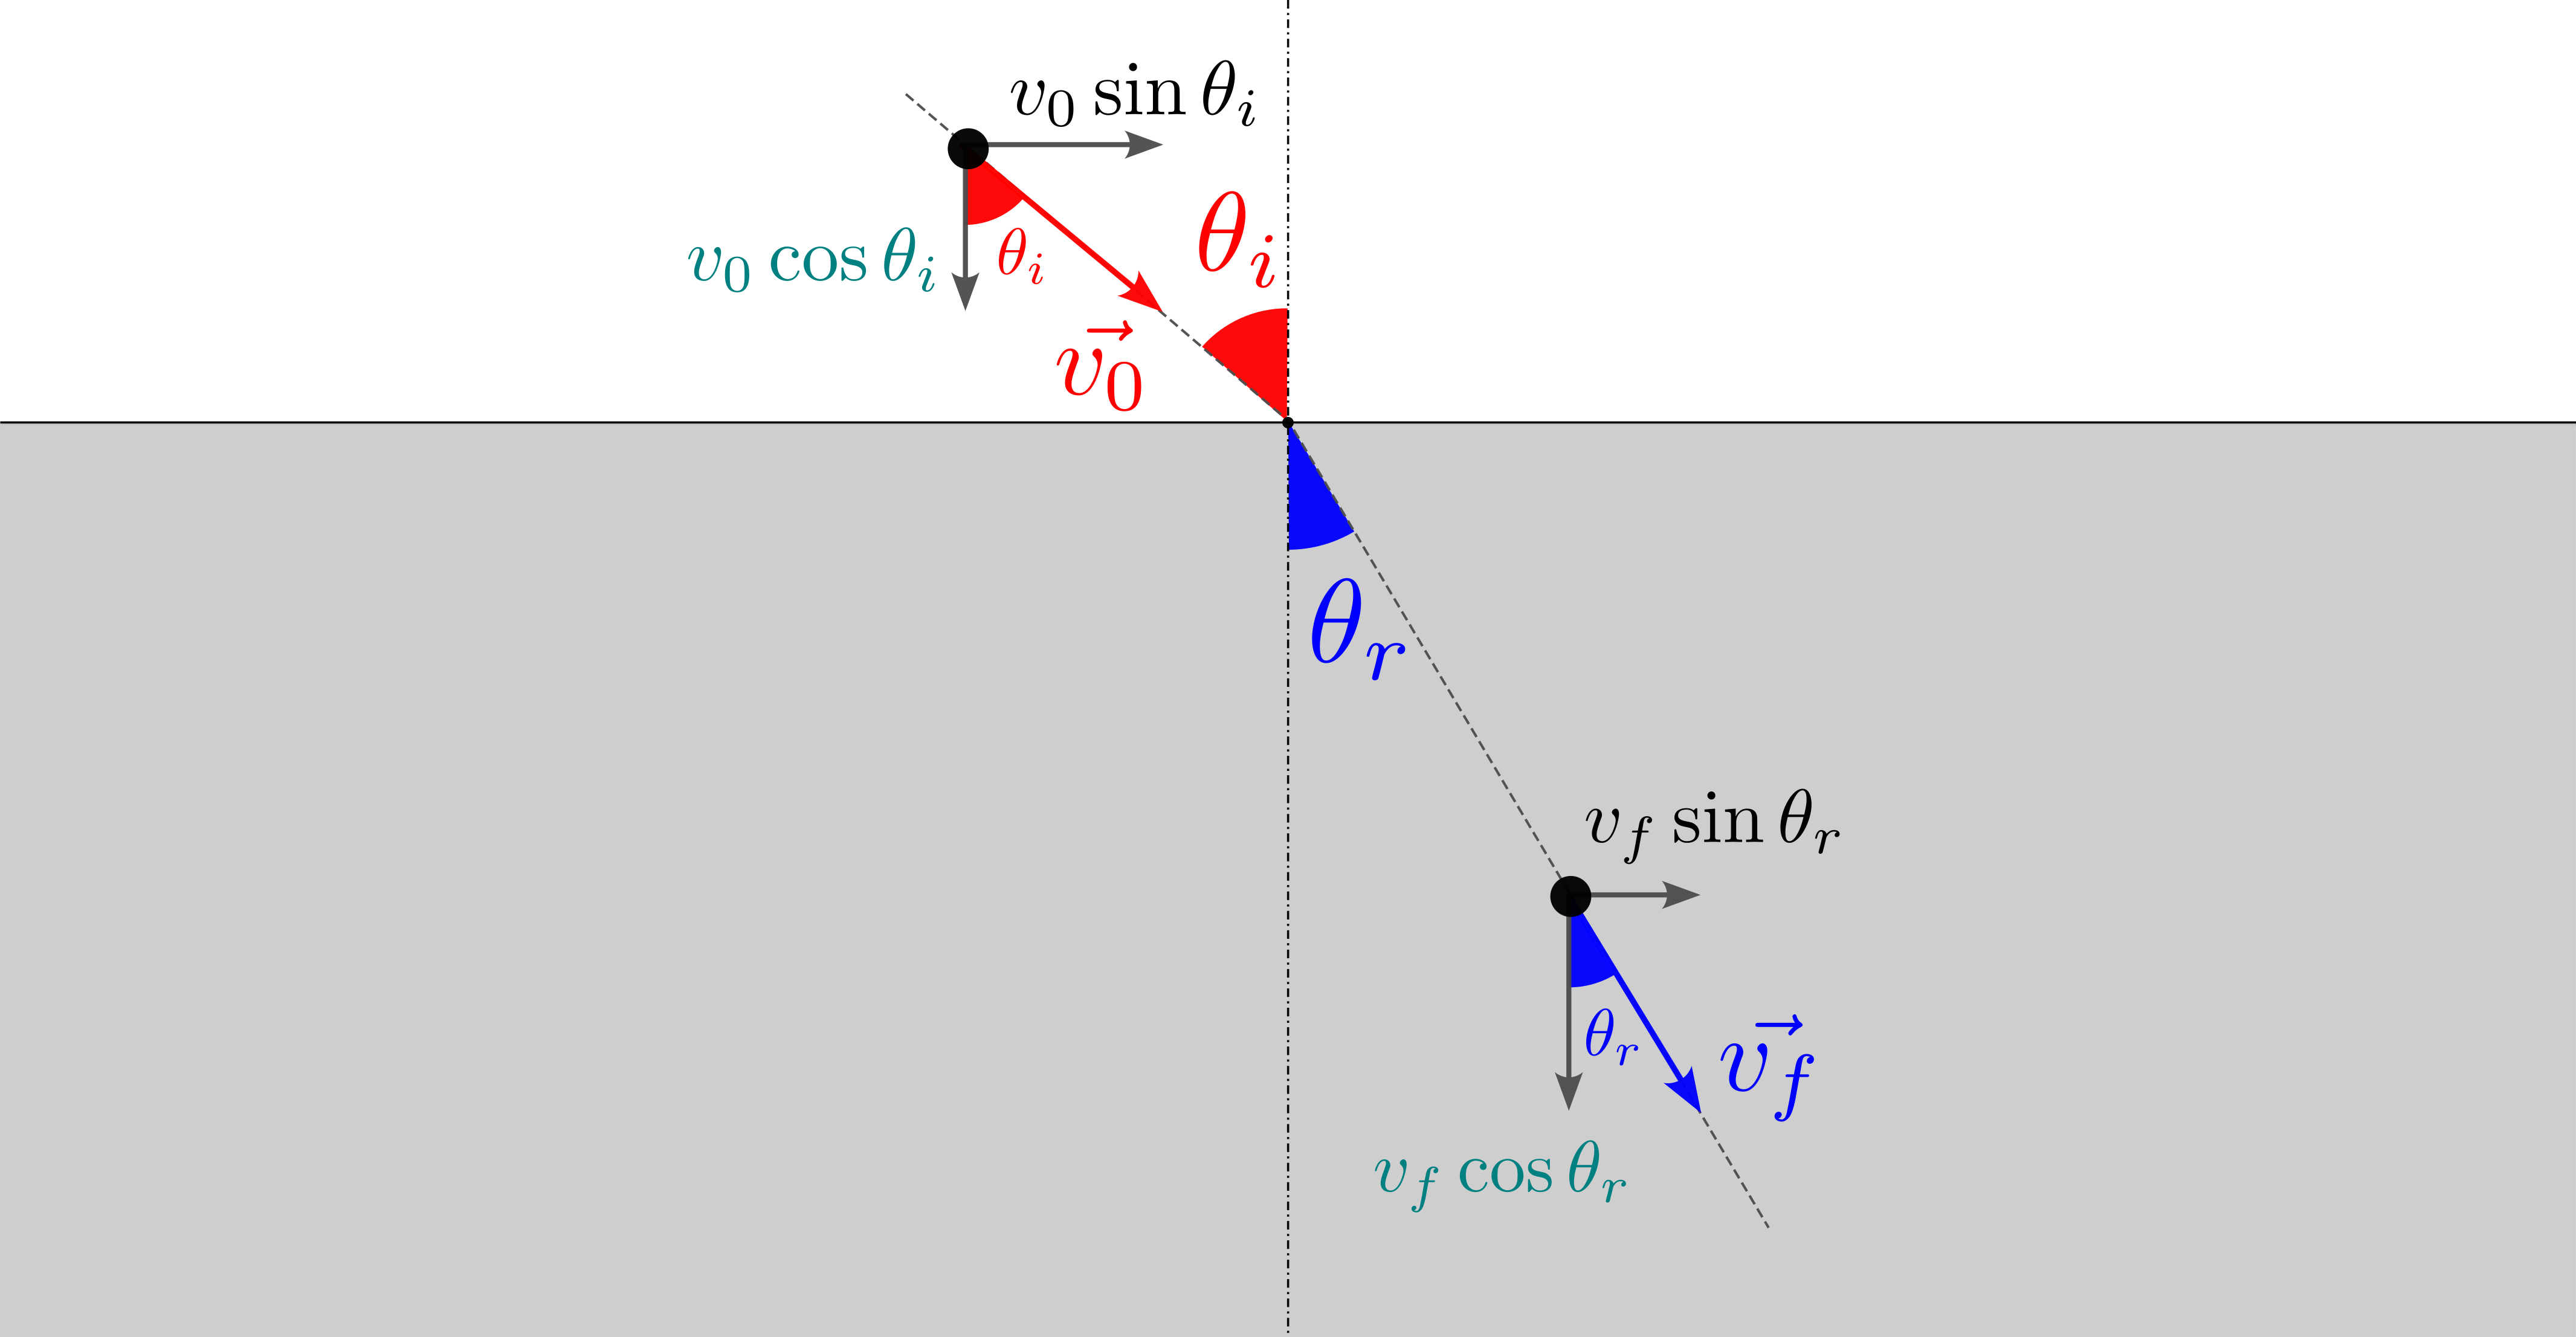
\includegraphics[width=0.8\textwidth]{img/refracao-newton.png}
        \caption{Refração corpuscular da luz.}
        \label{fig:refracao-newton}
    \end{figure}
    \vspace*{20pt}

    A componente horizontal não se altera, de modo que

    \begin{align}
        \begin{split}
            \frac{\sin\theta_i}{\sin\theta_r}&=\frac{v_f}{v_0}
        \end{split}
    \end{align}

    Sabendo que $\theta_i>\theta_r$, decorre que
    \begin{align}
        \frac{\sin\theta_i}{\sin\theta_r}&>1
    \end{align}

    como consequência
    \begin{align}
        v_f&>v_0
    \end{align}

    Ou seja, a velocidade da luz na água deve ser maior do que no ar.
    \end{proof}

    